\documentclass{beamer}
\usepackage{multicol}
\setlength{\columnsep}{0.5cm}

\mode<presentation>
{
  \usetheme{Darmstadt}   
  \usecolortheme{default} 
  \usefonttheme{default} 
  \setbeamertemplate{footline}[frame number]
  \setbeamertemplate{navigation symbols}{}
} 

\usepackage[english]{babel}
\usepackage[utf8x]{inputenc}

\title[Audition]{Candidature pour allocation doctorale}
\author{Quentin Garchery}
\date{Mardi 12 juin 2018}

\begin{document}

\begin{frame}
  \titlepage
\end{frame}


\section{Cursus universitaire}

\subsection{}

\begin{frame}{Cursus universitaire: 2009-2016}
\begin{itemize}
  \item 2009-2011 : MPSI à Jeanne d'Albret et MP$^*$  à Louis-le-Grand
  \item 2011-2016 : ENS Cachan, antenne de Bretagne\\
  \textbf{Stage de juin à juillet 2012 à l'IMJ} : \\
  \textit{Théorie additive des nombres}, Eric Balandraud \\
  \textbf{Stage de mai à juin 2014 à l'IMJ} : \\
  \textit{Représentation de groupes}, Olivier Brunat
  \item 2014-2015 : Préparation à l'agrégation de mathématiques \\
  \textit{rang 66$^e$ sur 274 admis}
  \item 2015-2016 : M2 mathématiques fondamentales à Paris Diderot \\
  \textbf{Stage de mai à août 2016 chez Eonos} : \\
  \textit{Algèbres de Clifford et application en informatique}, Thomas Dionysopoulos \\
  Programmation en Bash et en R
\end{itemize}
\end{frame}

\begin{frame}{Cursus universitaire: 2016-2018}
\begin{itemize}
  \item 2016-2017 : M1 Informatique parcours recherche à Paris Diderot\\
  \textbf{Travail de Recherche Encadré de mars à juin 2017} :\\
  \textit{Les systèmes distribués}, Gustavo Petri et Constantin Enea\\
  Vérification grâce à Alloy
  \vspace{5mm}
  \item 2017-2018 : M2 MPRI à Paris Diderot\\
  \textbf{Stage de mars à août 2018 au LRI} : \\
  \textit{Démonstration automatique en Coq}, Chantal Keller et Valentin Blot\\
  Programmation en OCaml et en Coq
\end{itemize}
\end{frame}


\section{Présentation du stage}

\subsection{}

\begin{frame}{Automatisation des assistants de preuve}
Les prouveurs automatiques : une source d'automatisation pour les assistants de preuve.
\begin{multicols}{2}
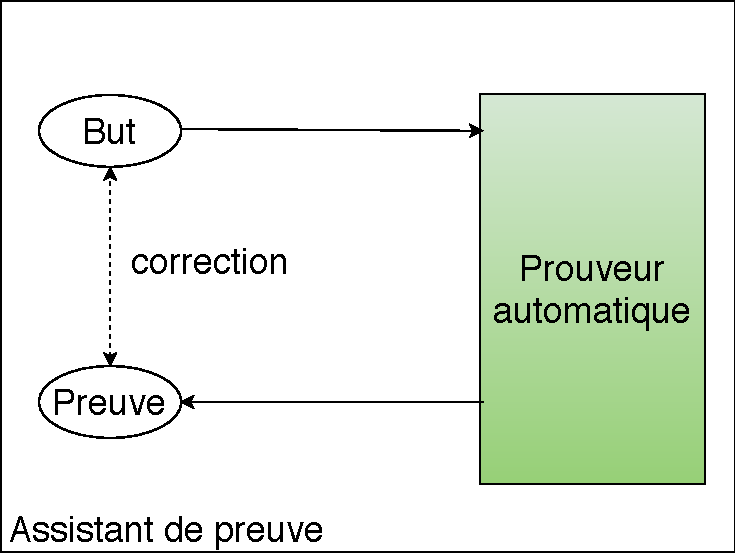
\includegraphics[height=4cm]{1_Autarcique.pdf}\\
Approche autarcique : vérifier le code du prouveur automatique.
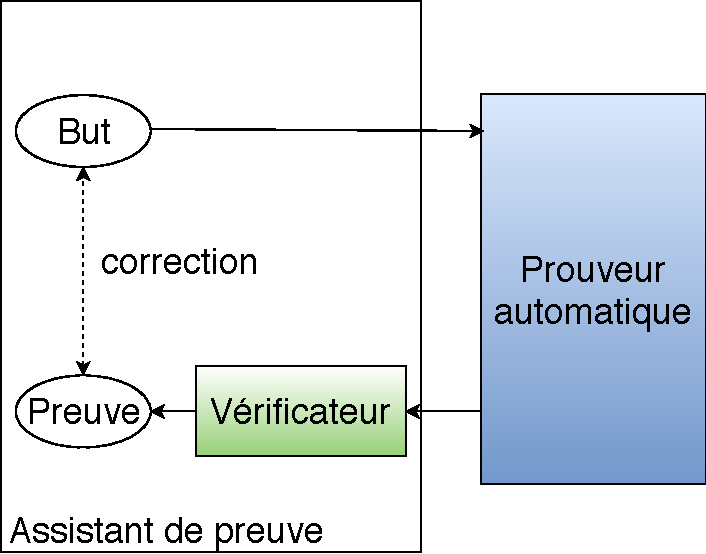
\includegraphics[height=4cm]{2_Sceptique.pdf}\\
Approche sceptique : vérifier la réponse du prouveur automati- que à chaque appel de celui-ci.
\end{multicols}
\end{frame}

\begin{frame}{Présentation de SMTCoq}
SMTCoq : une interface sceptique aux différents prouveurs automatiques actuellement développée par Chantal Keller en collaboration avec l'université d'Iowa. \\
\vspace*{7mm}
But : amélioration de l'automatisation de Coq et de la confiance dans les prouveurs automatiques. \\
\vspace*{7mm}
Sait prouver automatiquement le théorème suivant :
\[ \forall x \forall y \forall f. x \neq y + 1 \vee f(y) = f(x-1) \]
Fragment supporté : logique propositionnelle, arithmétique linéaire sur $\mathbb{Z}$, égalité et fonctions non-interprétées, vecteurs de bits, théorie des tableaux, variables quantifiées universellement en tête de formule.

\end{frame}

\begin{frame}{Amélioration de l'expressivité}
SMTCoq ne sait pas montrer que :
\[\forall h. homme(h) \Rightarrow mortel(h)\]
\[homme(Socrate)\]
implique :
\[mortel(Socrate)\]
\vspace*{2mm} \\
Objectifs du stage : permettre l'ajout de lemmes quantifiés au contexte et tenir compte de leurs instanciations dans le certificat.
\vspace*{6mm}\\
\end{frame}

\begin{frame}{Ajout de lemmes au contexte}
\begin{center}
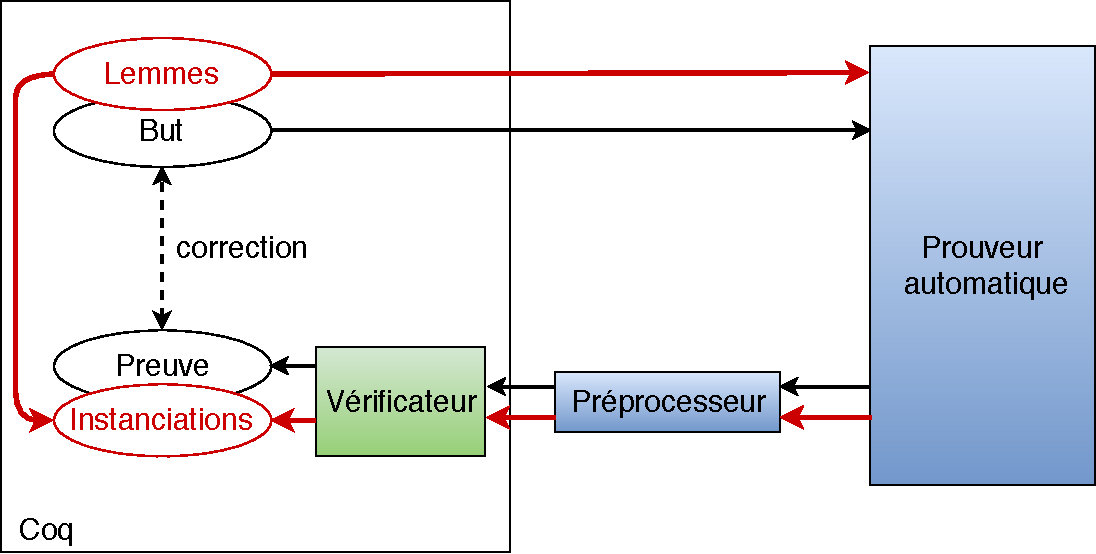
\includegraphics[height=5cm]{3_Contrib_Stage.pdf}
\end{center}
\end{frame}

\begin{frame}{Résultats du stage}
Vérificateur : s'appuie sur une preuve calculatoire en Coq. \\

\begin{block}{Théorème de correction}
$\forall l \, \forall c. \quad checker \, l \, c = true \quad \Rightarrow \quad interp \, l$
\end{block}
\vspace{3mm}
Un exemple en Coq :
\begin{center}
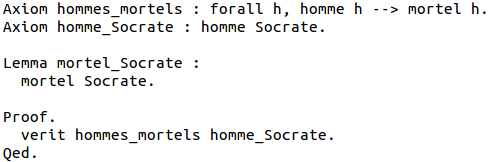
\includegraphics[height=2.5cm]{4_Socrate.png}
\end{center}
\vspace{3mm}
$\longrightarrow $ github.com/QGarchery/smtcoq-1
\end{frame}


\section{Motivation pour le sujet de thèse}

\subsection{}

\begin{frame}{Objectifs de la thèse}

\begin{itemize}
\item Améliorer la confiance dans les outils de preuve de programmes tels que Why3.
\vspace{5mm}
\item Certification de la génération et la transformation d'obligations de preuve par l'approche sceptique.
\end{itemize}



\end{frame}

\begin{frame}{Génération et vérification de certificats}
\begin{center}
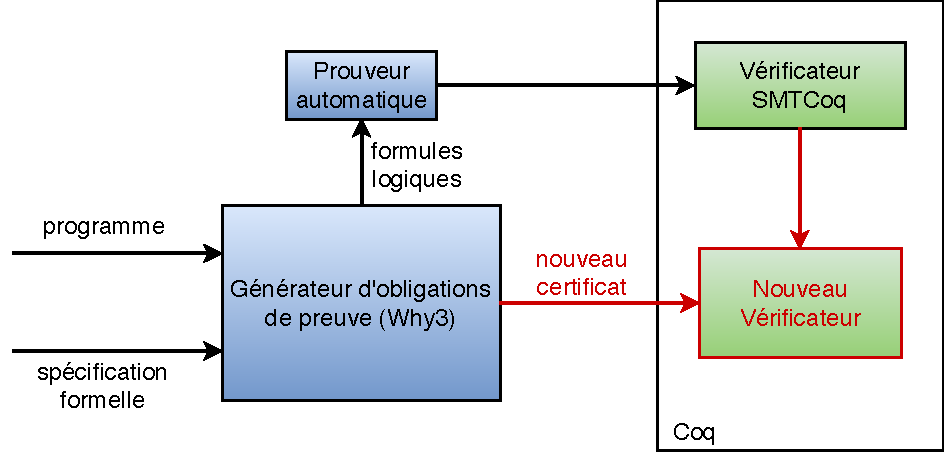
\includegraphics[height=5.2cm]{5_Contrib_These.pdf}
\end{center}
\end{frame}

\begin{frame}{Motivations personnelles}
\begin{itemize}
\item Certification : dans la continuité du sujet de stage.
\vspace{1cm}
\item EJCP 2018 à Lyon.
\vspace{1cm}
\item Sujet informatique en lien fort avec les mathématiques.
\end{itemize}
\end{frame}

\begin{frame}{Cadre de la thèse}
\begin{block}{\center{Certification de la génération et la transformation\\ d'obligations de preuve}}
\center{Claude Marché, Chantal Keller et Andrei Paskevich}
\end{block}
\vspace{7mm}
S'inscrit dans une collaboration entre le LRI et le CEA LIST sur la certification d'outils d'analyse de code C critique.

\end{frame}



\end{document}


























